\chapter{MiniML}

		\section{Syntaxe}
Ce langage est indépendant des langages que nous venons de voir. Nous pouvons tout de même le formaliser grâce à la notation BNF : \\
$E_F$ ::= $n$ $|$ $x$ $|$ fun $x$ -$>$ $E_F$ $|$ $E_F$ $E_F$ $|$ $E_F$ + $E_F$
\vspace{1\baselineskip} \\
De même, nous obtenons le système d'inférence suivant : \\
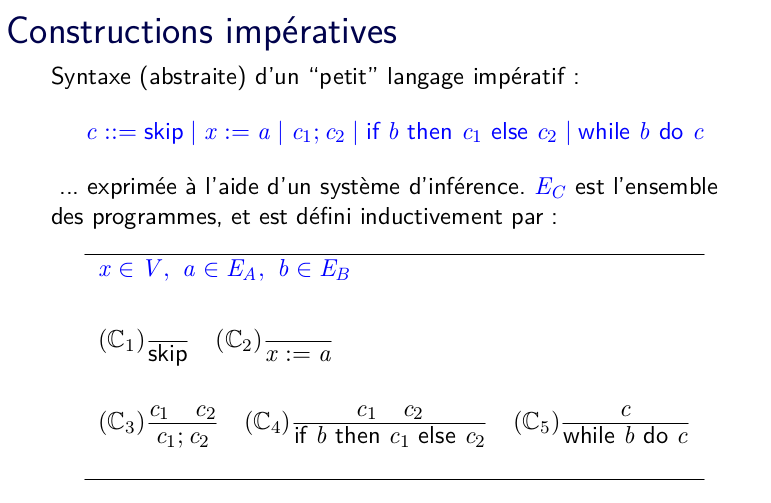
\includegraphics[height=4cm]{\MiniMLroot/definition_inductive.png} \\
A présent, nous allons pouvoir écrire des programmes fonctionnels !

	\subsection{Traduction en OCaml}

\lstinputlisting[language=OCaml, linerange={602-608}]{\OCamlroot/OCaml_exemple.ml}

\lstinputlisting[language=OCaml, linerange={631-648}]{\OCamlroot/OCaml_exemple.ml}

\lstinputlisting[language=OCaml, linerange={659-675}]{\OCamlroot/OCaml_exemple.ml}

\lstinputlisting[language=OCaml, linerange={688-694}]{\OCamlroot/OCaml_exemple.ml}



\lstinputlisting[language=OCaml, linerange={726-739}]{\OCamlroot/OCaml_exemple.ml}

\lstinputlisting[language=OCaml, linerange={748-754}]{\OCamlroot/OCaml_exemple.ml}


\lstinputlisting[language=OCaml, linerange={778-784}]{\OCamlroot/OCaml_exemple.ml}

\lstinputlisting[language=OCaml, linerange={790-797}]{\OCamlroot/OCaml_exemple.ml}

\lstinputlisting[language=OCaml, linerange={808-827}]{\OCamlroot/OCaml_exemple.ml}

\lstinputlisting[language=OCaml, linerange={840-846}]{\OCamlroot/OCaml_exemple.ml}

\lstinputlisting[language=OCaml, linerange={881-896}]{\OCamlroot/OCaml_exemple.ml}

\lstinputlisting[language=OCaml, linerange={905-911}]{\OCamlroot/OCaml_exemple.ml}



	
		\section{Appel par valeur}
		
		\subsection{Sémantique opérationnelle d’évaluation à grands pas}

\includegraphics[height=4cm]{\MiniMLroot/Appel_par_valeur/eval_grands_pas.png}		
		
		\subsection{Sémantique opérationnelle d’évaluation à petits pas}
		
\includegraphics[height=4cm]{\MiniMLroot/Appel_par_valeur/eval_petits_pas.png}		
		
		\section{Appel par nom}
		
		\subsection{Sémantique opérationnelle d’évaluation à grands pas}

\includegraphics[height=4cm]{\MiniMLroot/Appel_par_nom/eval_grands_pas.png}		
		
		\subsection{Sémantique opérationnelle d’évaluation à petits pas}

\includegraphics[height=4cm]{\MiniMLroot/Appel_par_nom/eval_petits_pas.png}